%%%%%%%%%%%%%%%%%%%%%%%%%%%%%%%%%%%%%%%%%%%%%%%%%%%%%%%%%%%%%%%%%%%%%%%%
\chapter{Traces}
\label{ch:trace}
%%%%%%%%%%%%%%%%%%%%%%%%%%%%%%%%%%%%%%%%%%%%%%%%%%%%%%%%%%%%%%%%%%%%%%%%

For simulations using \SIM, x86 traces are generated using Pin~\cite{pin} and
PTX traces are generated using GPUOcelot~\cite{ocelot}. Internally, \SIM
converts both x86 and PTX trace instructions into RISC style micro-ops (uop)
for simulation. Figure~\ref{fig:overview} shows a high-level overview of
this procedure. 

\begin{figure*}[htb]
\centering 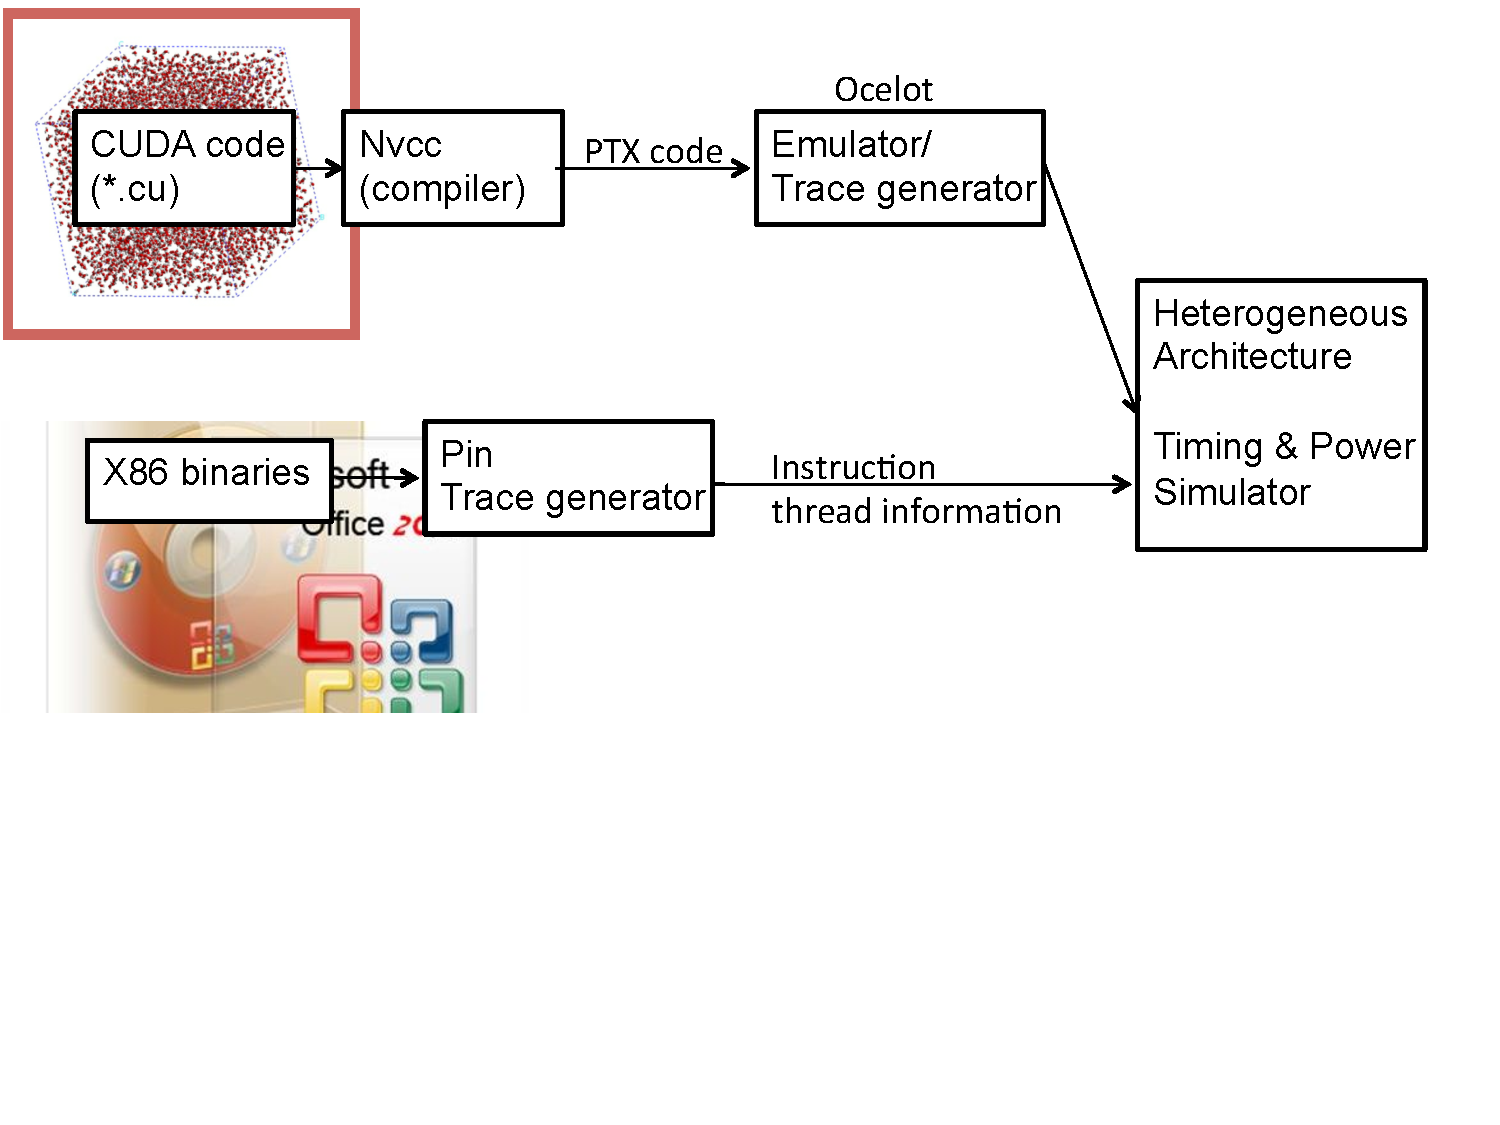
\includegraphics{figs/macsim_overview}
\caption{The overview of MacSim Traces Generation}
\label{fig:overview}
\end{figure*}


%%%%%%%%%%%%%%%%%%%%%%%%%%%%%%%%%%%%%%%%%%%%%%%%%%%%%%%%%%%%%%%%%%%%%%%%
%\section{Trace Generation}
%\label{sec:trace_generation}
%%%%%%%%%%%%%%%%%%%%%%%%%%%%%%%%%%%%%%%%%%%%%%%%%%%%%%%%%%%%%%%%%%%%%%%%



%%%%%%%%%%%%%%%%%%%%%%%%%%%%%%%%%%%%%%%%%%%%%%%%%%%%%%%%%%%%%%%%%%%%%%%%
\section{CPU (x86) Traces}
%%%%%%%%%%%%%%%%%%%%%%%%%%%%%%%%%%%%%%%%%%%%%%%%%%%%%%%%%%%%%%%%%%%%%%%%

\SIM includes a CPU (x86) trace generator which is based on Pin~\cite{pin}, a
binary instrumentation tool. Documentation regarding Pin can be found at
\urlc{http://www.pintool.org}. After installing Pin\footnote{Note that our
trace generator may not be backward/forward compatible with different Pin
versions. Currently, pin 2.12 (version number 56759  )  must be used.}, the x86
trace generator module has to be built. The command for doing so is:


\ignore
		{
		CPU (x86) traces are generated with the aid of Pin~\cite{pin}, a
		binary instrumentation tool.  Documentation regarding Pin can be found 
		here \urlc{http://www.pintool.org}.  We provide
		\cpu trace generator within \SIM repository. After installing
		Pin\footnote{Note that our CPU trace generator may not be
		  backward/forward compatible with the pin version. Currently, pin
		  41150 revision (Jun 07, 2011) must be used.}, we need to build the
		X86 trace generator module (trace\_generator.so), which can be simply
		done with the following commands.
		}



\begin{Verbatim}
cd toos/x86_trace_generator
make
\end{Verbatim}

\noindent This will generate trace\_generator.so in the
tools/x86\_trace\_generator/obj-intel64 directory. x86
traces for \SIM can then be generated by running Pin with the generated module.


\begin{Verbatim}
pin -t trace_generator.so -- $BIN $ARGS (for single-threaded applications)
pin -t trace_generator.so -thread N -- $BIN $ARGS (for multi-threaded applications with N threads)
\end{Verbatim}


The following example shows the generation of traces for an execution of /bin/ls. 

\begin{Verbatim}
pin -t trace\_generator.so -- /bin/ls
\end{Verbatim}


\noindent The binary (ls) is actually executed on top of Pin and the
instructions executed by the binary are written to the trace file. The output
on the screen when generating traces for \textit{ls} is shown.

\begin{Verbatim}
pin -t trace_generator.so -- /bin/ls
-> Thread[0->0] begins.
-> Trace Generation Starts at icount 0
dump.txt_0.dump  pin.log  trace_0.raw  trace_generator.o  trace_generator.so  
xed_extractor.o  xed_extractor.so
-> Trace Generation Done at icount 475195
\end{Verbatim}

The trace generator generates two files (in case of a single threaded
application) - Trace.txt and trace\_0.raw, in the current directory.
Section~\ref{sec:traceformat} provides details of the generated files.



%%%%%%%%%%%%%%%%%%%%%%%%%%%%%%%%%%%%%%%%%%%%%%%%%%%%%%%%%%%%%%%%%%%%%%%%
\section{GPU (PTX) Traces}
\label{sec:gpu_traces}
%%%%%%%%%%%%%%%%%%%%%%%%%%%%%%%%%%%%%%%%%%%%%%%%%%%%%%%%%%%%%%%%%%%%%%%%

GPU (PTX) traces are generated using GPUOcelot~\cite{ocelot}, a dynamic compilation
framework for heterogeneous systems. 


%%%%%%%%%%%%%%%%%%%%%%%%%%%%%%%%%%%%%%%%%%%%%%%%%%%%%%%%%%%%%%%%%%%%%%%%
\subsection{Installing Ocelot}
%%%%%%%%%%%%%%%%%%%%%%%%%%%%%%%%%%%%%%%%%%%%%%%%%%%%%%%%%%%%%%%%%%%%%%%%

Currently Ocelot can be download from github. Ocelot supports up to
CUDA 4.2 so higher CUDA versions need to be compiled with 4.2. 

\begin{Verbatim}
 git clone https://github.com/gtcasl/gpuocelot.git
\end{Verbatim}

A simple guide of compiling Ocelot to generate traces is provided 
at macsim/tools/ocelot\_install\_guide.txt. 
More detailed information is available at Ocelot's homepage. 

\ignore{
Then build Ocelot and the trace generator libraries.

\begin{Verbatim}
cd gpuocelot/ocelot; sudo ./build.py --install
cd gpuocelot/trace-generators; libtoolize; aclocal; autoconf; automake; ./configure; 
make; sudo make install
\end{Verbatim}

All libraries will be installed in the system library path directory
(\Verb+/usr/local/lib+). More detailed instructions for installing
Ocelot are available at Ocelot's Google Code project page.
}


%%%%%%%%%%%%%%%%%%%%%%%%%%%%%%%%%%%%%%%%%%%%%%%%%%%%%%%%%%%%%%%%%%%%%%%%
\subsection{Generating Traces}
%%%%%%%%%%%%%%%%%%%%%%%%%%%%%%%%%%%%%%%%%%%%%%%%%%%%%%%%%%%%%%%%%%%%%%%%

CUDA executables targeted for trace generation must be linked against
libocelot.so and libocelotTrace.so. libocelot.so provides the functionality of
the CUDA runtime library (libcudart.so) and libocelotTrace.so contains the
trace generator for \SIM and tools provided by Ocelot.

To execute a binary linked against libocelot.so a configuration file,
\Verb+configure.ocelot+ (which is in JSON format), is required in the same
directory as the binary. A copy of this file with some default settings can
be obtained from the Ocelot source. To enable trace generation, open your
copy of the configure.ocelot and add the pair \Verb+x86Trace: true+ on a new
line under the trace member as shown below.  Make sure that there is a comma
at the end of each pair that is not the last pair of a member.

\begin{Verbatim}
  trace: {
    database: "traces-ipdom/database.trace",
    memoryChecker: {
      enabled: true,
      checkInitialization: false
    },
    raceDetector: {
      enabled: true,
      ignoreIrrelevantWrites: true
    },
    cacheSimulator: {
      enabled: false,
    },
    branch: false,
    memory: false,
    x86Trace: true
  },
\end{Verbatim}

In addition to editing configure.ocelot, the following four environment
variables have to be set:

\begin{itemize}\itemsep2pt
\item[-] TRACE\_PATH : directory to store generated traces. If not specified, current directory is used by default.
\item[-] TRACE\_NAME : prefix used in the file name for generated traces. If not specified, "Trace" is used by default.
\item[-] KERNEL\_INFO\_PATH : name of file that should contain kernel information (must be specified)
\item[-] COMPUTE\_VERSION : compute capability (default 2.0)
\end{itemize}


Examples for setting up these environment variables are shown below.

\begin{Verbatim}
export TRACE_PATH="/storage/traces/"  # Create a trace directory in the /storage/traces
export KERNEL_INFO_PATH="kernel_info" # kernel_info has the kernel information
export COMPUTE_VERSION="2.0"          # Calculate occupancy based on compute capability 2.0
\end{Verbatim}

On executing the binary of a kernel, an information file and a directory for each
kernel invocation by the binary are generated. These directories contain traces from 
different invocations of the kernel. The directories path are addressed by \Verb+TRACE\_PATH+. 
The kernel information file contains the version of generated traces and path of
each trace configuration file. The trace configuration file contains the number of warps, the
trace version, maximum number of thread blocks that can be assigned to each SM
and the ID, and starting information of each warp. More information regarding
the generated files can be found in Sections~\ref{sec:traceformat} and ~\ref{sec:kern_config}. 

\ignore
		{
		The kernel information file (kernel\_info) should contain the following
		information: kernel name, register usage (per thread), and shared memory usage
		(per thread).


		\begin{Verbatim}
		_Z9Memcpy_SWPfS_i 14 52 
		\end{Verbatim}


		Running CUDA application creates a directory with the kernel name, where traces 
		are generated, and kernel\_config.txt which is a configuration used for MacSim.


		\begin{Verbatim}
		drwxr-xr-x   2 anonymous group 69632 Sep 00 22:03 _Z9Memcpy_SWPfS_i_0
		-rw-r--r--   1 anonymous group    66 Sep 09 22:29 kernel_config.txt
		\end{Verbatim}
		}


%%%%%%%%%%%%%%%%%%%%%%%%%%%%%%%%%%%%%%%%%%%%%%%%%%%%%%%%%%%%%%%%%%%%%%%%
\section{Supporting Other Architectures}
%%%%%%%%%%%%%%%%%%%%%%%%%%%%%%%%%%%%%%%%%%%%%%%%%%%%%%%%%%%%%%%%%%%%%%%%

To support other ISAs such as ARM, a frontend simulator or a
functional emulator is necessary to provide the executed instruction stream. 
Instructions in this stream can be translated by \SIM into
its internal RISC style micro-ops and simulated. Currently, plans for
supporting ARM ISA and OpenGL programs are in progress.


%%%%%%%%%%%%%%%%%%%%%%%%%%%%%%%%%%%%%%%%%%%%%%%%%%%%%%%%%%%%%%%%%%%%%%%%
\section{Trace Formats}
\label{sec:traceformat}
%%%%%%%%%%%%%%%%%%%%%%%%%%%%%%%%%%%%%%%%%%%%%%%%%%%%%%%%%%%%%%%%%%%%%%%%

\paragraph{Note:}

\textit{Although different trace generators use the same data structure for
storing instruction traces, the meaning of some of the members of this
common data structure is different in PTX traces. Note that efforts to
have different data structures for x86 and PTX traces for sake of
extensibility and clarity are underway.}


On a successful trace generation, the x86 trace generator generates a
configuration file called Trace.txt and one Trace\_xx.raw file
(assuming that \Verb+TRACE\_PATH+ was set to "Trace") for each thread
of the application in the output directory. On the other hand, the PTX
trace generator generates a kernel information file and several
directories containing traces of individual kernel invocations. The
directory for each kernel invocation contains a Trace.txt file and one
Trace\_xx.raw file for each warp in the kernel.  Note that in case of
PTX kernels, one trace file is generated for each warp, there are no
per thread trace files. Further details regarding trace generation for
PTX kernels can be found in Section~\ref{sec:ptx_traces}. The purposes
of Trace.txt and Trace\_xx.raw are shown below and their formats are
explained in detail in subsequent sections.


\begin{itemize}\itemsep2pt
\item Trace.txt (info trace): contains information about the generated
  trace files (\#threads, trace type, ...).

\item Trace\_xx.raw (raw trace): contains instruction trace for a
  thread and is generated for each thread.\footnote{In case of GPU, a
    warp is mapped to a \SIM thread, where a warp consists of 32
    threads in CUDA.}
\end{itemize}



%%%%%%%%%%%%%%%%%%%%%%%%%%%%%%%%%%%%%%%%%%%%%%%%%%%%%%%%%%%%%%%%%%%%%%%%
\subsection{Trace.txt}
%%%%%%%%%%%%%%%%%%%%%%%%%%%%%%%%%%%%%%%%%%%%%%%%%%%%%%%%%%%%%%%%%%%%%%%%


\begin{figure*}[htb]
\centering
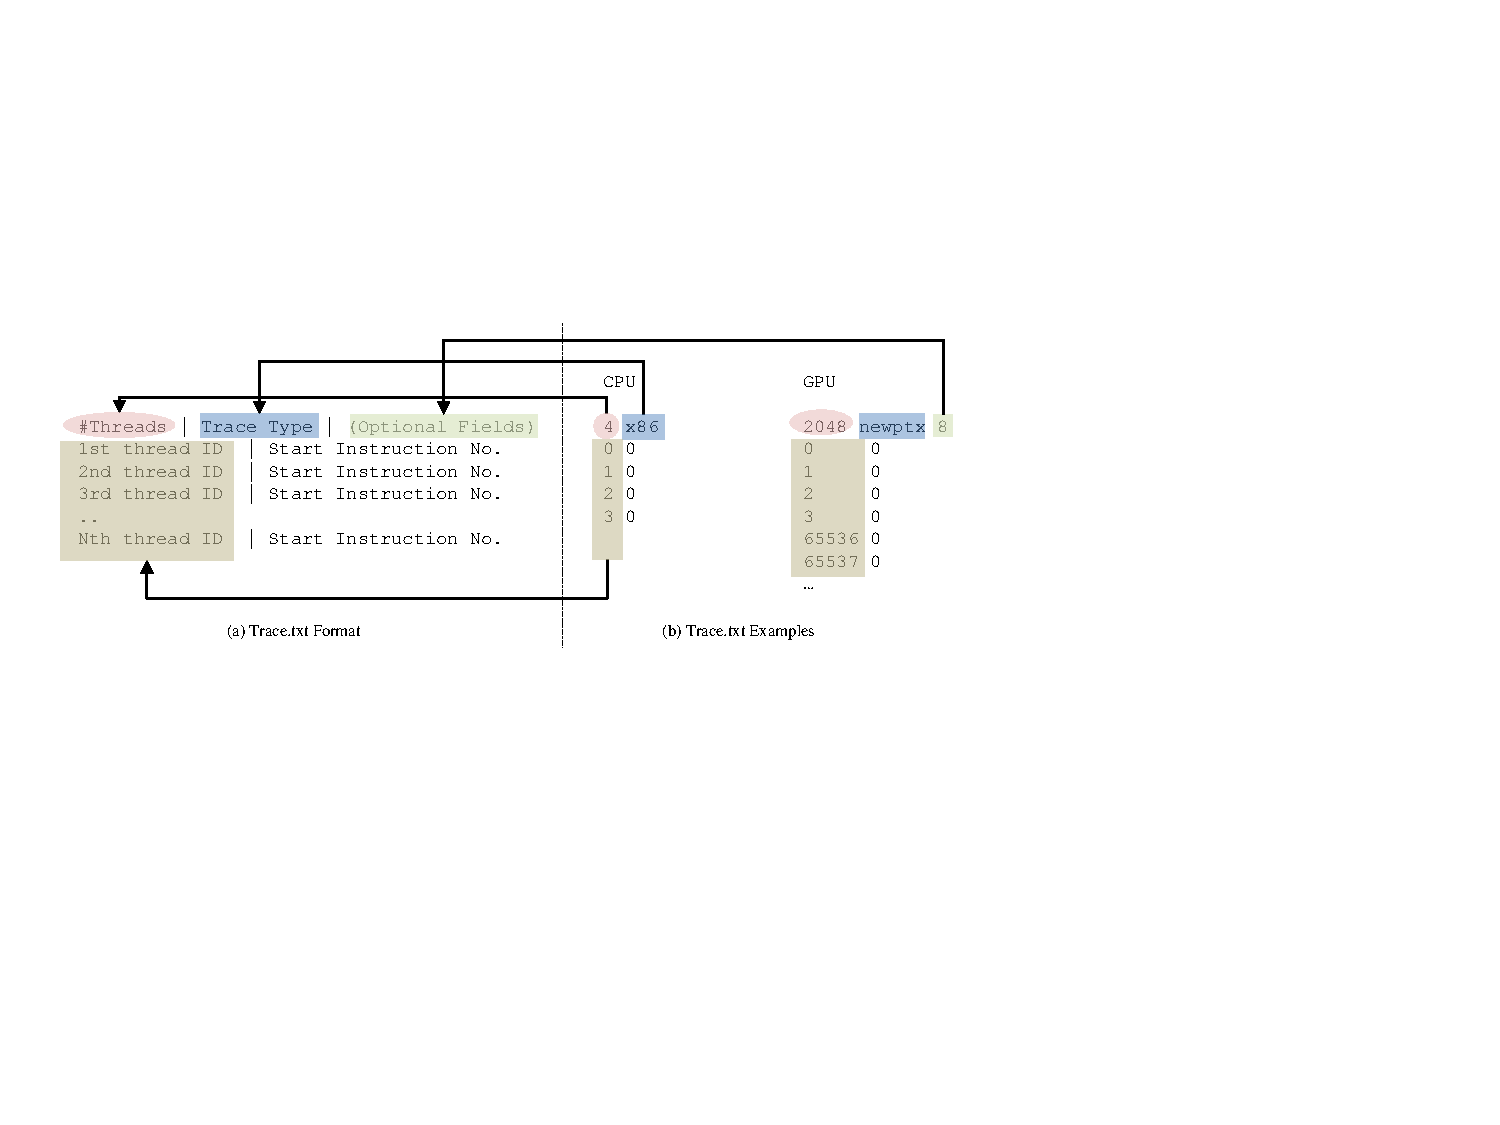
\includegraphics{figs/trace_format}
\caption{Trace.txt format}
\label{fig:trace_format}
\end{figure*}


Figure~\ref{fig:trace_format}-(a) shows the format of Trace.txt and its CPU and GPU
examples.  As shown in Figure~\ref{fig:trace_format}-(a), the first line in
Trace.txt has different fields from the rest of the lines.

\begin{itemize}\itemsep2pt
\item \#Threads: indicates the number of threads for which traces have
  been generated, and this value is equal to the number of lines in
  the file excluding the first line.
\item Trace Type: indicates whether the generated traces are for an
  x86 application or a PTX kernel.
\item Optional Field(s): currently used for PTX traces only and
  indicates the number of thread blocks that can be assigned to a
  streaming multiprocessor(SM) core (occupancy).
\end{itemize}

From the second line onwards, there are two fields in each line:
thread id and start instruction number. For each thread, there is a
Trace\_<thread\_id>.raw file which contains the dynamic instruction
trace for the thread. Finally, start instruction number indicates when
each thread should be started in terms of the number of instructions
simulated for the main thread of the application. In a PTX kernel
since all warps are ready for execution at the launch of the kernel,
the start instruction number for all threads is zero. On the other
hand, for a x86 application, the start instruction is non-zero for all
threads except thread 0, which is the main (or parent) thread in the
application. This is because in most multi-threaded CPU applications,
main thread (thread id 0) spawns children threads.


In Figure~\ref{fig:trace_format}-(b), the CPU trace has four threads and its
type is set to x86. The ids of the threads are 0-3 with the corresponding trace
files being Trace\_0.raw$-$Trace\_3.raw . Thread 0 is ready at the start of
simulation, while Threads 1, 2 and 3 become ready when Thread 0 has fetched x,
y and z instructions respectively.


In the GPU example, the number of traces files is 2048 since \#Threads
(representing \#Warps in case of GPUs) is 2048.  The optional field indicates
that eight thread blocks can be assigned to a SM core. 

For GPU traces, the id in the file encodes thread block information as
well. The warp id and thread block id can be decoded from this id as follows:

\begin{Verbatim}
warp_id  = id % (1 << 16)
block_id = id / (1 << 16)
\end{Verbatim}

\ignore
		{
		In the GPU trace, thread ID is calculated by thread block ID * 65536 + warp ID (in a block). 
		In the example, warps 0, 1, 2 and 3 are comprised of a thread block, and warps 65536, 65537, 65538
		and 65539 forms another thread block.
		}

%%%%%%%%%%%%%%%%%%%%%%%%%%%%%%%%%%%%%%%%%%%%%%%%%%%%%%%%%%%%%%%%%%%%%%%%
\subsection{Trace\_xx.raw}
%%%%%%%%%%%%%%%%%%%%%%%%%%%%%%%%%%%%%%%%%%%%%%%%%%%%%%%%%%%%%%%%%%%%%%%%

Trace\_xx.raw is generated for each thread/warp and contains the
dynamic instruction trace for the thread/warp in binary
format. The structure/format for encoding instructions is the same in
both x86 and PTX traces and looks like as follows (in order):


%trace format for an instruction in trace_xx.raw

\vspace{0.2in}
\begin{footnotesize}
\begin{tabular}{l c l l}
Type            & Size (Bytes) & Field                     & Description                                            \\ \hline \hline
\Verb+uint8_t+  & 1            & \Verb+m_num_read_regs+    & number of source registers                             \\
\Verb+uint8_t+  & 1            & \Verb+m_num_dest_regs+    & number of destination registers                        \\
\Verb+uint8_t+  & 9            & \Verb+m_src[MAX_SRC_NUM]+ & source register IDs                                    \\
\Verb+uint8_t+  & 6            & \Verb+m_dst[MAX_DST_NUM]+ & destination register IDs                               \\
\Verb+uint8_t+  & 1            & \Verb+m_cf_type+          & branch type                                            \\
\Verb+bool+     & 1            & \Verb+m_has_immediate+    & indicates whether this instruction has immediate field \\
\Verb+uint8_t+  & 1            & \Verb+m_opcode+           & opcode                                                 \\
\Verb+bool+     & 1            & \Verb+m_has_st+           & indicates whether this instruction has store operation \\
\Verb+bool+     & 1            & \Verb+m_is_fp+            & indicates whether this instruction is a FP operation   \\
\Verb+bool+     & 1            & \Verb+m_write_flg+        & write flag                                             \\
\Verb+uint8_t+  & 1            & \Verb+m_num_ld+           & number of load operations                              \\
\Verb+uint8_t+  & 1            & \Verb+m_size+             & instruction size                                       \\
\Verb+uint32_t+ & 4            & \Verb+m_ld_vaddr1+        & load address 1                                         \\
\Verb+uint32_t+ & 4            & \Verb+m_ld_vaddr2+        & load address 2                                         \\
\Verb+uint32_t+ & 4            & \Verb+m_st_vaddr+         & store address                                          \\
\Verb+uint32_t+ & 4            & \Verb+m_instruction_addr+ & PC address                                             \\
\Verb+uint32_t+ & 4            & \Verb+m_branch_target+    & branch target address                                  \\
\Verb+uint8_t+  & 1            & \Verb+m_mem_read_size+    & memory read size                                       \\ 
\Verb+uint8_t+  & 1            & \Verb+m_mem_write_size+   & memory write size                                      \\
\Verb+bool+     & 1            & \Verb+m_rep_dir+          & repetition direction                                   \\
\Verb+bool+     & 1            & \Verb+m_actually_taken+   & indicates whether branch is actually taken             \\
\end{tabular}
\end{footnotesize}
\vspace{0.2in}


Note that the raw trace is compressed with zlib to reduce the sizes of
the generated trace files, and the size of each field is the size
before the compression.


%%%%%%%%%%%%%%%%%%%%%%%%%%%%%%%%%%%%%%%%%%%%%%%%%%%%%%%%%%%%%%%%%%%%%%%%
\subsection{kernel\_config.txt (only for PTX)}
\label{sec:kern_config}
%%%%%%%%%%%%%%%%%%%%%%%%%%%%%%%%%%%%%%%%%%%%%%%%%%%%%%%%%%%%%%%%%%%%%%%%

For PTX traces, as described in Section~\ref{sec:gpu_traces}, a directory is
created for each kernel invocation, where Trace.txt and Trace\_xx.raw are
generated. Since typical GPU applications usually invoke several kernels (or
execute the same kernel repeatedly), PTX traces can have multiple kernel
directories. Thus, in order to simulate all invoked kernels for a GPU
application, the PTX trace generator creates kernel\_config.txt which contains
information of the invoked kernels.


\begin{Verbatim}
Contents of output directory after trace generation

ll /trace/ptx/parboil/bfs

drwxr-xr-x  4  4096 Sep 21 13:21 .
drwxr-xr-x 11  4096 Sep 13 18:02 ..
drwxr-xr-x  2  4096 Apr  7  2011 _Z17BFS_in_GPU_kernelPiS_P4int2S1_S_S_iS_ii_0
drwxr-xr-x  2  4096 Apr  7  2011 _Z26BFS_kernel_multi_blk_inGPUPiS_P4int2S1_S_S_S_S_iiS_S_S__0
-rw-r--r--  1   184 Apr  7  2011 kernel_config.txt

In kernel_config.txt

-1 newptx
/trace/ptx/parboil/bfs/_Z17BFS_in_GPU_kernelPiS_P4int2S1_S_S_iS_ii_0/Trace.txt
/trace/ptx/parboil/bfs/_Z26BFS_kernel_multi_blk_inGPUPiS_P4int2S1_S_S_S_S_iiS_S_S__0/Trace.txt
\end{Verbatim}


As shown above, all the invoked kernels are enumerated in kernel\_config.txt.
The first line indicates that this is a wrapper file which points to (multiple)
trace.txt files, one for each kernel invocation. \SIM reads and simulates the
traces sequentially, one kernel at a time.  In the above example (bfs),
kernel\_config.txt indicates that there are two different kernels in bfs,
each of which was invoked once. When running a GPU simulation, the path to
the kernel\_config.txt file is specified trace\_file\_list
(Section~\ref{sec:run}).  Also, we can simulate specific kernels
by modifying the kernel\_config.txt file.

%%%%%%%%%%%%%%%%%%%%%%%%%%%%%%%%%%%%%%%%%%%%%%%%%%%%%%%%%%%%%%%%%%%%%%%%
\subsection{Translation into micro-ops}
%%%%%%%%%%%%%%%%%%%%%%%%%%%%%%%%%%%%%%%%%%%%%%%%%%%%%%%%%%%%%%%%%%%%%%%%

During simulation, each instruction in a \emph{raw trace} file is
converted into one or more micro-ops internally. \SIM stores such
decoded micro-uops in the \SIM-specific structure shown in
Table~\ref{table:trace_uops}.

\begin{table*}[!htb]
\begin{footnotesize}
\begin{center}
\caption{\SIM-specific data structure for micro-ops.}
\label{table:trace_uops}
\begin{tabular}{|l|l|l|} 
\hline
Type      & Variable                 & Description \\ \hline \hline
uint8\_t  & m\_opcode                & opcode \\ \hline
Uop\_Type & m\_op\_type              & type of operation \\ \hline
Mem\_Type & m\_mem\_type             & type of memory instruction \\ \hline
Cf\_Type  & m\_cf\_type              & type of control flow instruction \\ \hline
Bar\_Type & m\_bar\_type             & type of barrier caused by instruction \\ \hline
uns       &   m\_num\_dest\_regs     & number of destination registers written \\ \hline
uns       &   m\_num\_src\_regs      & number of source registers read \\ \hline
uns       &   m\_mem\_size           & number of bytes read/written by a memory instruction \\ \hline
uns       &   m\_inst\_size          & instruction size \\ \hline
Addr      &   m\_addr                & PC address  \\ \hline
reg\_info\_s&   m\_srcs[MAX\_SRCS]   & source register information \\ \hline
reg\_info\_s&   m\_dests[MAX\_DESTS] & destination register information \\ \hline
Addr      &   m\_va;                 & virtual address \\ \hline
bool      &   m\_actual\_taken       & branch actually taken \\ \hline
Addr      &   m\_target              & branch target address \\ \hline
Addr      &   m\_npc                 & next PC address  \\ \hline
bool      &   m\_pin\_2nd\_mem       & has second memory operation \\ \hline
inst\_info\_s& *m\_info              & pointer to the instruction hash table  \\ \hline
int       &   m\_rep\_uop\_num       & repeated uop number \\ \hline
bool      &   m\_eom                 & end of macro \\ \hline
bool      &   m\_alu\_uop            & ALU uop  \\ \hline
uint32\_t  &   m\_active\_mask       & active mask \\ \hline
uint32\_t  &   m\_taken\_mask        & branch taken mask \\ \hline
Addr      &   m\_reconverge\_addr    & address of reconvergence \\ \hline
bool      &   m\_mul\_mem\_uops      & multiple memory transactions \\ \hline

\end{tabular}
\end{center}
\end{footnotesize}
\end{table*}

\ignore{
		The following shows the data structure for micro-uops. 
		\begin{Verbatim}
		  uint8_t      m_opcode;        /**< opcode */
		  Uop_Type     m_op_type;       /**< type of operation */
		  Mem_Type     m_mem_type;      /**< type of memory instruction */
		  Cf_Type      m_cf_type;       /**< type of control flow instruction */ 
		  Bar_Type     m_bar_type;      /**< type of barrier caused by instruction */
		  uns          m_num_dest_regs; /**< number of destination registers written */
		  uns          m_num_src_regs;  /**< number of source registers read */
		  uns          m_mem_size;      /**< number of bytes read/written by a memory instruction */
		  uns          m_inst_size;     /**< instruction size */
		  Addr         m_addr;          /**< pc address */ 
		  reg_info_s   m_srcs[MAX_SRCS]; /**< source register information */
		  reg_info_s   m_dests[MAX_DESTS]; /**< destination register information */
		  Addr         m_va;            /**< virtual address */
		  bool         m_actual_taken;  /**< branch actually taken */
		  Addr         m_target;        /**< branch target address */
		  Addr         m_npc;           /**< next pc address */ 
		  bool         m_pin_2nd_mem;   /**< has second memory operation */
		  inst_info_s *m_info;          /**< pointer to the instruction hash table */ 
		  int          m_rep_uop_num;   /**< repeated uop number */
		  bool         m_eom;           /**< end of macro */
		  bool         m_alu_uop;       /**< alu uop */ 
		  // GPU simulation
		  uint32_t     m_active_mask;   /**< active mask */
		  uint32_t     m_taken_mask;    /**< branch taken mask */
		  Addr         m_reconverge_addr; /**< address of reconvergence */
		  bool         m_mul_mem_uops;  /**< multiple memory transactions */
		\end{Verbatim}
}

% LocalWords:  GPU PTX gpuocelot

%%%%%%%%%%%%%%%%%%%%%%%%%%%%%%%%%%%%%%%%%%%%%%%%%%%%%%%%%%%%%%%%%%%%%%%%%%%%%%%%%%%%%%

\ignore
		{
		\begin{table*}[htb]
		\begin{footnotesize}
		\begin{center}
		\caption{MacSim trace format.}
		\label{table:trace_format}
		\begin{tabular}{|l|l|} 
		\hline
		Type               & Description \\ \hline 
		uint8\_t           & number of source registers \\ \hline
		uint8\_t           & number of destination registers \\ \hline
		uint8\_t[9]        & source register IDs \\ \hline
		uint8\_t[6]        & destination register IDs \\ \hline
		uint8\_t           & branch type \\ \hline
		bool               & indicates whether this instruction has immediate field \\ \hline
		uint8\_t           & opcode \\ \hline
		bool               & indicates whether this instruction has store operation \\ \hline
		bool               & indicates whether this instruction is FP operation \\ \hline
		bool               & write flag \\ \hline
		uint8\_t           & number of load operations \\ \hline
		uint8\_t           & instruction size \\ \hline
		uint32\_t          & load address 1 \\ \hline
		uint32\_t          & load address 2 \\ \hline
		uint32\_t          & store address \\ \hline
		uint32\_t          & PC address \\ \hline
		uint32\_t          & branch target address \\ \hline
		uint32\_t          & memory read size \\ \hline
		uint8\_t           & memory write size \\ \hline
		uint8\_t           & repetition direction  \\ \hline
		uint8\_t           & indicates whether branch is actually taken \\ \hline

		\end{tabular}
		\end{center}
		\end{footnotesize}
		\end{table*}
		}

\ignore
		{
		\begin{table*}[htb]
		\begin{footnotesize}
		\begin{center}
		\caption{MacSim trace format.}
		\label{table:trace_format}
		\begin{tabular}{|l|l|l|l|l|l|l|l|l|l|l|l|l|l|l|l|} 
		\hline
		nSR & nDR & SR\_IDs & DR\_IDs & BrType & bImm & Opcode & bStore & bFP & WF & nLD  \\ \hline \hline
		InstSize & LAddr\_1 & LAddr\_2 & SAddr & PCAddr & BrAddr & MemRSize & MemWSize & RepDir & BrActT & \\ \hline
		\end{tabular}
		\end{center}
		\end{footnotesize}
		\end{table*}

		Tables~\ref{table:trace_format} and ~\ref{table:trace_desc} show the trace
		format for each instruction and the description of each field, respectively.
		}

 